\chapter{Solving the challenge}

In order to solve the challenge you will only need:
\begin{itemize}
	\item{Understanding how integer overflows and truncation work in memory (at bit level).}
	\item{Understanding the size of primitive data types matter and, even though \code{int}'s size may vary, on most modern compilers it is 32 bits~\cite{QuoraDataTypesSizes, NewCIntegerC99}.}
	\item{A calculator with bit-view mode, and preferably bit-toggling capabilities, in order to help you visualize what is actually happening. Windows10's default calculator in Programmer mode/view is awesome. As a Linux alternative you can use KCalc\footnote{\url{https://kde.org/applications/utilities/org.kde.kcalc}}.}
\end{itemize}

\begin{figure}[h]
	\makebox[\textwidth][c]{
		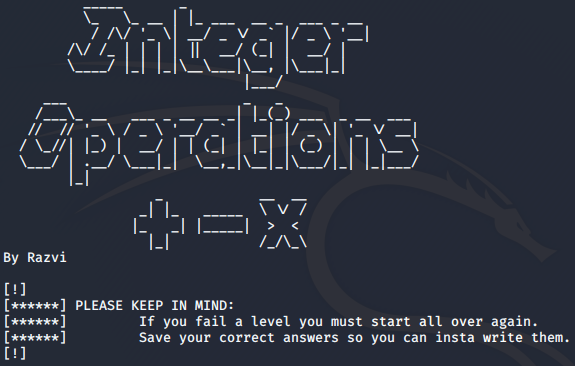
\includegraphics{binary_intro.png}
	}
	\label{fig:binary_intro}
	\caption{Binary's introduction.}
\end{figure}

%%%%%%%%%%%%%%%%%%%%%%%%%%%%%%%%%%%%%%%%%%%%%%%%%%%%%%%%%%%
\section{Level 1: Basics of addition}

\begin{figure}[!htbp]
	\makebox[\textwidth][c]{
		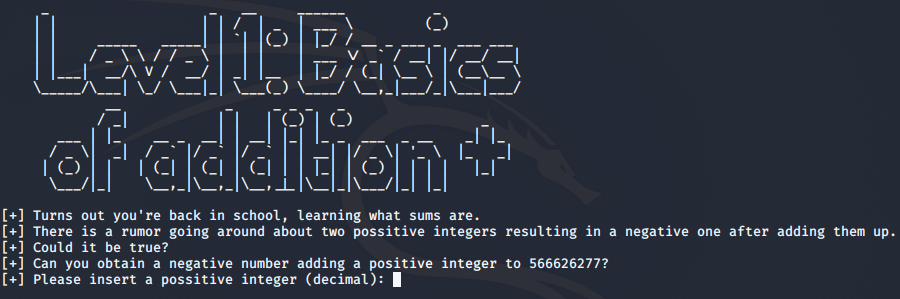
\includegraphics[scale=.8]{intro_level1.png}
	}
	\caption{Formulation of the first level.}
	\label{fig:intro_level1}
\end{figure}

The level's description states that two positive integers could result in a negative one after adding them up. It sounds like a signedness bug resulting from an arithmetic operation, i.e., the  addition.

Every time you run the binary it will ask you about a different, random number. To pass the level you can either provide a solution of that particular number or look for a general solution that works with every single time. So far, the only thing we know for sure is that the program will give you a positive integer, in the example shown in Figure~\ref{fig:intro_level1} it is 1659611044, and you must insert another positive one. So far we can assume that internally the program is working with \code{signed int} data types because otherwise a negative result would be impossible. 

As you may already know, when working with \code{signed int} the most significant bit (the leftmost bit) is the one that indicates the sign. If it is set, the number is negative. Figure~\ref{fig:bit_representation} shows the bit representation of both a positive (a) and a negative (b) number.

\begin{figure}
	\begin{subfigure}[t]{.5\textwidth}
		\centering
		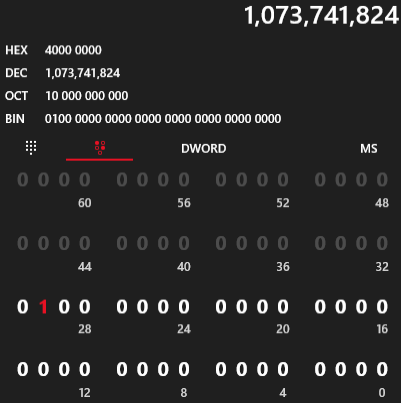
\includegraphics[width=\textwidth]{bit_positive.png}
		\caption{Positive integer}
		\label{fig:sub_positive_int}
	\end{subfigure}
	\begin{subfigure}[t]{.5\textwidth}
		\centering
		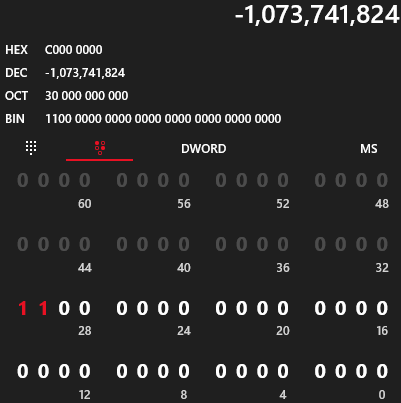
\includegraphics[width=\textwidth]{bit_negative.png}
		\caption{Negative integer}
		\label{fig:sub_negative_int}
	\end{subfigure}
	\caption{32 bit representation of integer}
	\label{fig:bit_representation}
\end{figure}


If you want to further read about how the CPU deals with positive and negative numbers you must read about \textbf{\textit{Two's complement}}~\cite{TwosComplementWikipedia,lyon1976two}.

In order to solve the level you must realize that the most significant bit must be set after the addition. That is, insert a number that added to the one given by the program results in any other integer whose most significant bit is set. Since the program will always generate a positive integer to be added with, there is a general solution for this level. That number is:
\begin{quote}
	Decimal: 2147483647\\
	Hex: 0x7FFFFFFF\\
	Binary: Figure~\ref{fig:solution_level_1}
\end{quote}

\begin{figure}
	\centering
	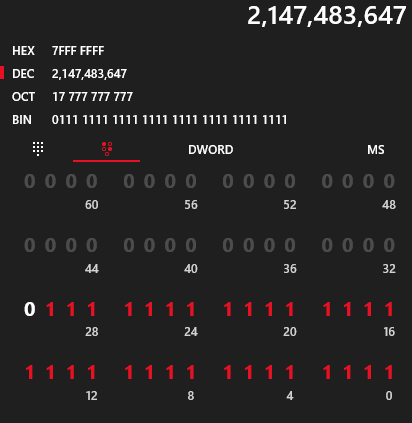
\includegraphics{solution_level1.png}
	\caption{General solution to level 1.}
	\label{fig:solution_level_1}
\end{figure}

It works no matter the positive integer given by the program because of the binary representation of the number 2147483647. It does not matter what other positive integer in the range $[1, 2147483647]$ is added to it, it will always result in a number with the 31st bit set, that is, a negative number. \textit{Please remember an integer \code{int} is 32 bits long, hence the max value 2147483647.}

You can write 2147483647 as the answer for the first level and it will always work. This number is \code{INT\_MAX} since it is the maximum positive value that can be stored in a \code{signed int} variable.
\begin{figure}
	\makebox[\textwidth][c]{
		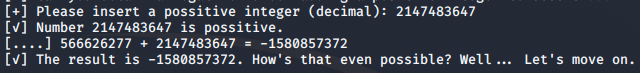
\includegraphics[scale=1]{solved_level1.png}
	}
	\caption{Solving the first level.}
	\label{fig:solved_level1}
\end{figure}
\clearpage
%%%%%%%%%%%%%%%%%%%%%%%%%%%%%%%%%%%%%%%%%%%%%%%%%%%%%%%%%%%%s
\section{Level 2: Basics of subtraction}

\begin{figure}[!htbp]
	\makebox[\textwidth][c]{
		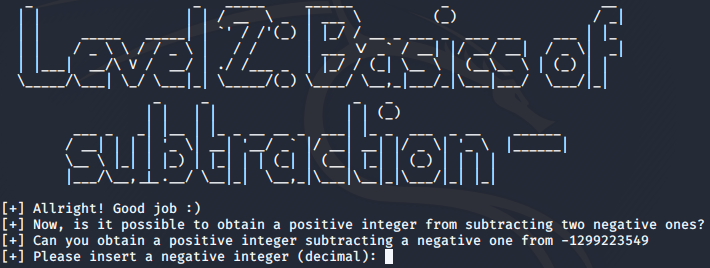
\includegraphics{intro_level2.png}
	}
	\caption{Formulation of the second level.}
	\label{fig:intro_level2}
\end{figure}

The second level is exactly the opposite to the first one, i.e., getting a positive number from the subtraction of two negative integers. Just like the first level, every time you run the binary the program will give you a different negative integer to subtract from. Just like before, you can solve the second level by either enter a solution for the particular case or finding a general solution that works with every single negative integer. 

Once again, it is of vital importance to think about the numbers in their binary form. Keep in mind that, as seen in Figure~\ref{fig:sub_negative_int}, a negative number has the most important bit set. In the context of the binary, since we are dealing with \code{int}s, that is the 31st bit set. We know the program will always generate a negative random number. That means the number we must subtract a negative integer from will always have the 31st bit set. What we must find now is an integer that added to the one provided by the program results in  number whose 31st bit is not set. Before continuing please notice I said \textit{added} and not subtracted because I find it easier to understand the concepts thinking about sum of bits rather than subtraction. It is equally valid to talk about summing two negative integers since the following are two equivalent arithmetic operations:
\begin{align*}
-1337 - 1000 = -2337\\
-1337 + (-1000) = -2337
\end{align*}

Now, in order to find a general solution we must figure out which is the negative number that no matter what negative integer it is added to, the result will always be positive (the most significant bit is not set). The solution is:
\begin{quote}
	Decimal: -2147483648\\
	Hex: 0x80000000\\
	Binary: Figure~\ref{fig:solution_level_2}
\end{quote}

\begin{figure}
		\centering
		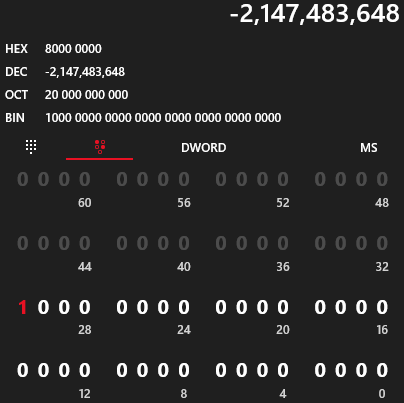
\includegraphics{solution_level2.png}
		\caption{General solution to level 2.}
		\label{fig:solution_level_2}
\end{figure}

It works because the only bit that is set in its binary representation is the most significant one. That means no matter what other negative integer in the range $[-1, -2147483648]$ it is added to since both numbers will have their most significant bit set. The result will be a number with the most significant bit not set, i.e., positive.  

You can write -2147483648 (with the minus sign) as the answer for the second level and it will always work. This number is \code{INT\_MIN} since it is the minimum value that can be stored in a \code{signed int} variable. 
\begin{figure}
	\makebox[\textwidth][c]{
		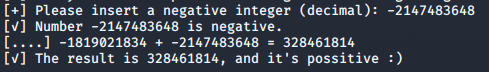
\includegraphics{solved_level2.png}
	}
	\caption{Solving the second level.}
	\label{fig:solved_level2}
\end{figure}
\clearpage
%%%%%%%%%%%%%%%%%%%%%%%%%%%%%%%%%%%%%%%%%%%%%%%%%%%%%%%%%%%%%%
\section{Level 3: Simple equations}

\begin{figure}[!htpb]
	\makebox[\textwidth][c]{
		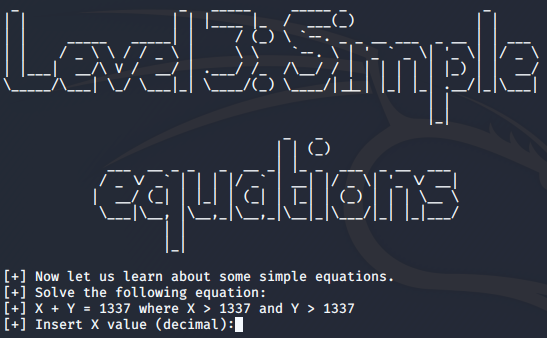
\includegraphics{intro_level3.png}
	}
	\caption{Formulation of the third level.}
	\label{fig:intro_level3}
\end{figure}

The third level presents a simple equation that must be solved. The equation is:

\begin{equation*}
	\left.\begin{aligned}
			X &> 1337\\
			Y &> 1337\\
			X + Y &= 1337	
	\end{aligned}
	\right\}
\end{equation*}

At a first glance it seems impossible to solve the equation since there is no way $X + Y = 1337$ when both $X$ and $Y$ are greater than $1337$. Unsurprisingly enough, there are plenty of alternative solutions to the equation given the context we are working in. Bear in mind we are working with \code{int}s that are 32 bits long. That is, there will be truncation after the sum. 

Given the binary representation of the number $1337$, as shown in Figure~\ref{fig:1337_binary}, we must find two integers both bigger than $1337$ that after adding them up, the first 32 bits of the result are equal to $1337$. The reasoning behind it is that only the first 32 bits will prevail in memory, the rest will be discarded (that is what truncation is). 

As long as both integers are bigger than $1337$ and their addition results in a number whose 32 first bits are  also $1337$, the solution is valid. That is why there are plenty of solutions to this level. I will show you the easiest solution but it is not the only one. 

The solution I used to pass the level consists in preserving the first 32 bit with the value $1337$ and simply setting the bit number 33 for the X value, and then unset all bits except the 33rd for the Y value. The logic behind it is truncation based, as mentioned earlier. Since all numbers will be truncated to the first 32 bits because we are working with \code{int}s.

\begin{figure}[!h]
	\centering
	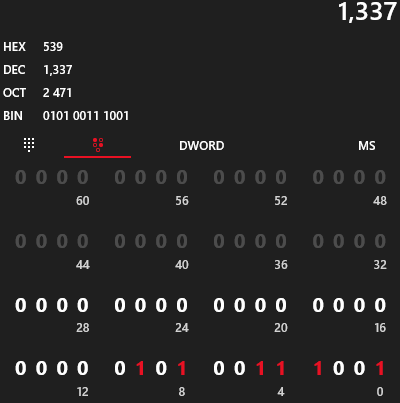
\includegraphics{level3_1337.png}
	\caption{Binary representation of $1337$.}
	\label{fig:1337_binary}
\end{figure}

\begin{figure}
	\begin{subfigure}[t]{.5\textwidth}
		\centering
		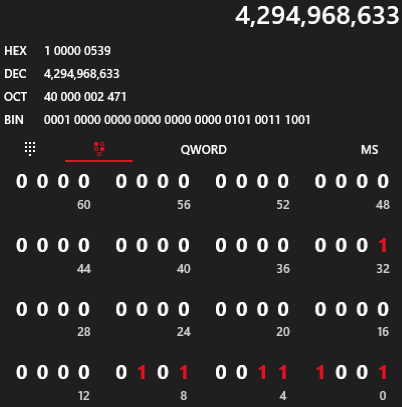
\includegraphics[width=\textwidth]{level3_solution_x.png}
		\caption{Bit representation of X value.}
	\end{subfigure}
	\begin{subfigure}[t]{.5\textwidth}
		\centering
		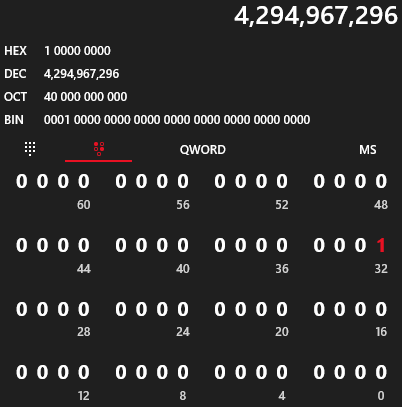
\includegraphics[width=\textwidth]{level3_solution_y.png}
		\caption{Bit representation of Y value.}
	\end{subfigure}
	\begin{subfigure}[t]{\textwidth}
		\centering
		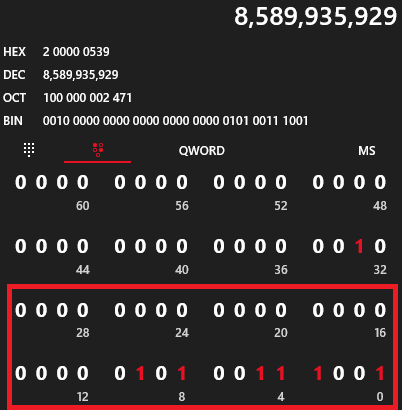
\includegraphics{level3_solution_x+y.png}
		\caption{Bit representation of the addition of X and Y.}
	\end{subfigure}
	\caption{Bit representation of one possible solution to level 3. Only the first 32 bits will prevail after truncation.}
\end{figure}

After inserting $42949686333$ value for $X$ and $4294967296$ for $Y$, the level is completed. It works because when a number such as  $42949686333$ does not fit into a 32 bit long \code{int} data type, so it gets truncated. The work-flow of the level is the following:
\begin{enumerate}
	\item{The user is asked for input for $X$ variable. User inserts $42949686333$. It is bigger than $1337$. Program tries to store it into an \code{int} variable. The number does not fit. It gets truncated to 32 bit. $X = 1337$ after truncation. }
	\item{The user is asked for input for $Y$ variable. User inserts $4294967296$. It is bigger than $1337$. Program tries to store it into an \code{int} variable. The number does not fit. It gets truncated to 32 bit. $Y = 0$ after truncation.}
	\item{$X = 1337; Y = 0; X + Y = 1337$. Level passed. }
\end{enumerate}


\begin{figure}[!h]
	\makebox[\textwidth][c]{
		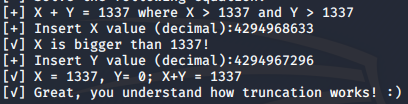
\includegraphics[scale=1]{solved_level3.png}
	}
	\caption{Solving the third level.}
	\label{fig:solved_level3}
\end{figure}
\clearpage
%%%%%%%%%%%%%%%%%%%%%%%%%%%%%%%%%%%%%%%%%%%%%%%%%%%%%%%%%%
\section{Level 4: Twisting the numbers}

\begin{figure}[!htbp]
	\makebox[\textwidth][c]{
		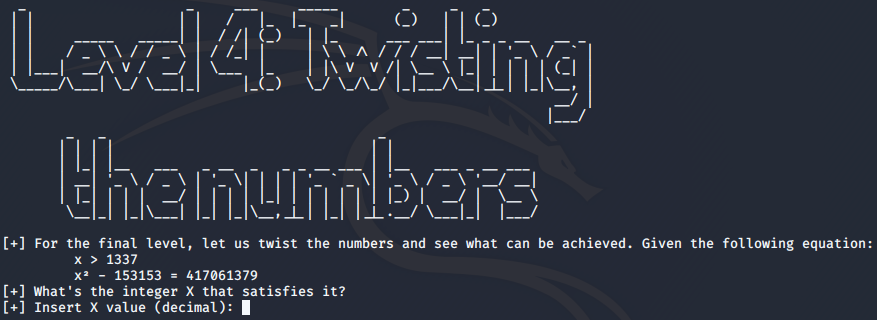
\includegraphics[scale=.85]{intro_level4.png}
	}
	\caption{Formulation of the forth and last level.}
	\label{fig:intro_level4}
\end{figure}

The forth and last level asks the user to solve a bit more complicated equation. The equation is:
\begin{equation*}
	\left.\begin{aligned}
		X &> 1337\\
		X^2 - 153153 &= 417061379
	\end{aligned}
	\right\}
\end{equation*}

Once again, the provided integer for $X$ must be bigger than 1337. In this case, this condition is irrelevant. This leaves us with the following equation:
\begin{equation*}
	X^2 - 153153 = 417061379
\end{equation*}

Now, isolating the X variable:
\begin{equation*}
	\begin{aligned}
		X &= \sqrt{417214532}; then\\
		X &= 20425.83002
	\end{aligned}
\end{equation*}

Well, this approach is incorrect. Remember we are working with integers, so there are no decimals. While it is true that $20425.83002^2 + 153153 \approx 417061379$, it is not a valid solution. The approach that must be followed is different since, in order to solve the challenge, truncation must be taken into account.  

What we know so far is that the program expects an integer that will be squared, subtracted $153153$ and then compared with $417061379$. That is, there must be some integer $X$ that complies with $X^2 = 417214532$. We have seen earlier that getting the square root of the number is not valid. 

Once again, we must think about binary representation of the numbers involved in this operation. The binary representation of $417214532$ is shown in Figure~\ref{fig:level4_bit_representation}. What we are looking for is a number that after multiplying it by itself, i.e., squaring it, the first 32 bits of the result represent the number $417214532$. In other words, we are looking for a number whose first 32 bits represent the number $417214532$ and the result of its square root is a valid integer. The result of the square root is the $X$ we are looking for. 

The number that meets the previous conditions is $17597083716$ whose representation can be seen in Figure~\ref{fig:level4_bit_representation2}. Please remember that we were looking for a number whose square root is a perfect integer and $\sqrt{17597083716} = 132654$. The answer to the level is $132654$.

Notice how $132654$ meets level's conditions. It is bigger than $1337$. $132654^2$ is $17597083716$. The number is stored in a \code{int} variable and gets truncated to 32 bits. $17597083716$ truncated is $417214532$. This leaves us with  $417214532 - 153153$ and it indeed is $417061379$. 

Insert $132654$ as the answer to level 4 and now level and whole challenge will be completed. 
\begin{figure}
	\begin{subfigure}[t]{.5\textwidth}
		\centering
		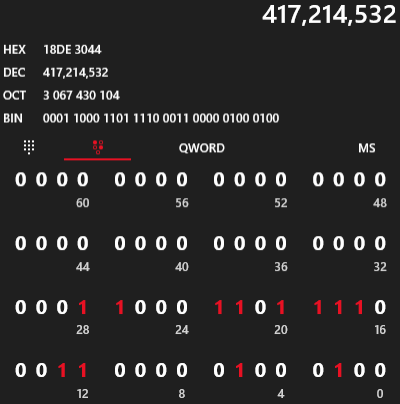
\includegraphics[width=\textwidth]{level4_bit_representation1.png}
		\caption{Bit representation of the expected result.}
		\label{fig:level4_bit_representation}
	\end{subfigure}
	\begin{subfigure}[t]{.5\textwidth}
		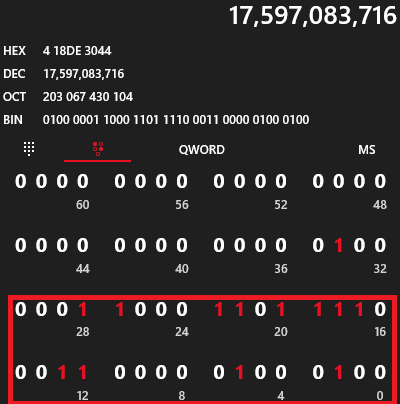
\includegraphics[width=\textwidth]{level4_bit_representation2.png}
		\caption{Bit representation of the result of squaring $X$. Only the first 32 bits will prevail after truncation.}
		\label{fig:level4_bit_representation2}
	\end{subfigure}
	\caption{Binary representations of numbers involved in level 4.}
\end{figure}

\begin{figure}[!h]
	\makebox[\textwidth][c]{
		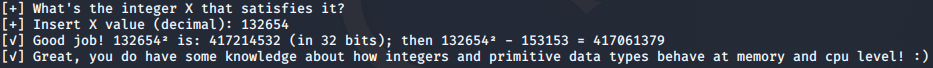
\includegraphics[scale=.8]{solved_level4.png}
	}
	\caption{Solving the forth and last level.}
	\label{fig:solved_level4}
\end{figure}